% ------------------------------------------------------------------------------
% TYPO3 Version 9.3 - What's New - Chapter "Introduction" (English Version)
%
% @author	Michael Schams <schams.net>
% @license	Creative Commons BY-NC-SA 3.0
% @link		http://typo3.org/download/release-notes/whats-new/
% @language	English
% ------------------------------------------------------------------------------
% LTXE-CHAPTER-UID:		7fdf26cc-362160ab-d6c8b905-19722b20
% LTXE-CHAPTER-NAME:	Introduction
% ------------------------------------------------------------------------------

\section{Introduzione}
\begin{frame}[fragile]
	\frametitle{Introduzione}

	\begin{center}\huge{Introduzione}\end{center}
	\begin{center}\huge{\color{typo3darkgrey}\textbf{I fatti in breve}}\end{center}

\end{frame}

% ------------------------------------------------------------------------------
% LTXE-SLIDE-START
% LTXE-SLIDE-UID:		6508cf57-1456d7e6-1693f3a8-df1c3ed4
% LTXE-SLIDE-TITLE:		TYPO3 Version 9.3 - The Facts
% ------------------------------------------------------------------------------
\begin{frame}[fragile]
	\frametitle{Introduzione}
	\framesubtitle{TYPO3 CMS Versione 9.3 - I fatti in breve}

	\begin{itemize}
		\item Data di rilascio: 12 Giugno 2018
		\item Tipo di rilascio: Sprint Release
	\end{itemize}

	\begin{figure}
		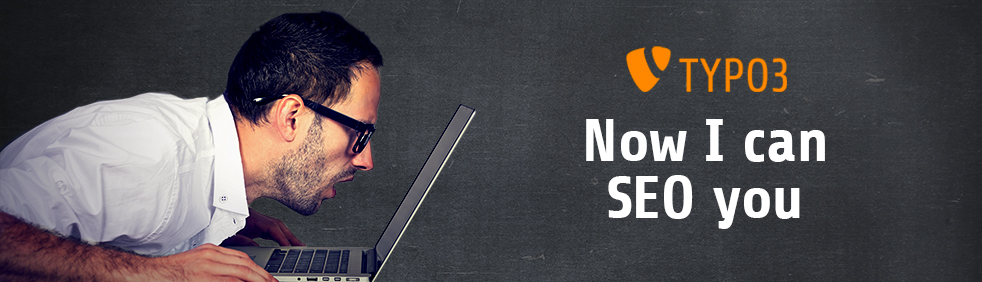
\includegraphics[width=0.95\linewidth]{Introduction/typo3-v93-banner.jpg}
	\end{figure}

\end{frame}

% ------------------------------------------------------------------------------
% LTXE-SLIDE-START
% LTXE-SLIDE-UID:		072956b8-ed81268b-c3121623-6d14f42f
% LTXE-SLIDE-TITLE:		System Requirements
% ------------------------------------------------------------------------------
\begin{frame}[fragile]
	\frametitle{Introduzione}
	\framesubtitle{Requisiti di sistema}

	\begin{itemize}
		\item PHP versione 7.2\newline
			\smaller
				(potrebbe essere ridotto a PHP 7.1 o 7.0 nelle prossime release, in attesa di decisione)
			\normalsize

		\item PHP settings:

			\begin{itemize}
				\item \texttt{memory\_limit} >= 128M
				\item \texttt{max\_execution\_time} >= 240s
				\item \texttt{max\_input\_vars} >= 1500
				\item l'opzione di compilazione \texttt{-}\texttt{-disable-ipv6} \underline{non} deve essere usata
			\end{itemize}

		\item La maggior parte dei Database supportati da \textbf{Doctrine DBAL} funzionano anche con TYPO3.
			I DB verificati sono ad esempio:
	\end{itemize}

	\begin{figure}
		
\includegraphics[width=0.70\linewidth]{Introduction/logo-databases.png}
	\end{figure}

\end{frame}

% ------------------------------------------------------------------------------
% LTXE-SLIDE-START
% LTXE-SLIDE-UID:		30cd846e-500098d6-64d98018-da67bf34
% LTXE-SLIDE-TITLE:		Development, Release and Maintenance Timeline
% ------------------------------------------------------------------------------
\begin{frame}[fragile]
	\frametitle{Introduzione}
	\framesubtitle{Sviluppo e tempi di rilascio}

	\textbf{TYPO3 v9}

	\begin{figure}
		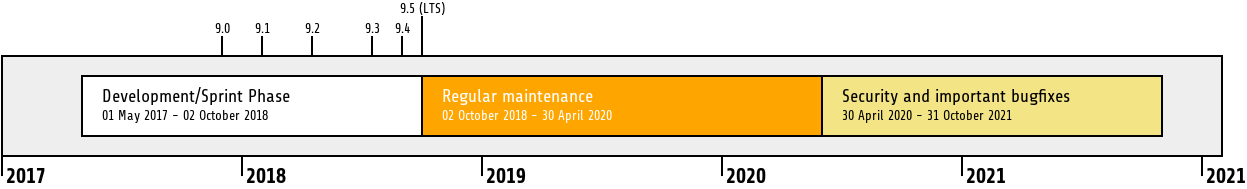
\includegraphics[width=1\linewidth]{Introduction/typo3-v9-lifecycle.png}
	\end{figure}

	\textbf{Estensione del supporto}\newline
	\smaller
		La \href{https://typo3.com}{TYPO3 GmbH} offre ulteriori opzioni di supporto
		per TYPO3 v9 LTS anche dopo il 31 ottobre 2021, per ulteriori due anni.
	\normalsize

%	\url{https://typo3.com/our-services/extended-support/}

\end{frame}

% ------------------------------------------------------------------------------
% LTXE-SLIDE-START
% LTXE-SLIDE-UID:		0a0f31a2-b5f379e3-a046a298-1b19a6d9
% LTXE-SLIDE-TITLE:		TYPO3 v9 Roadmap
% ------------------------------------------------------------------------------
\begin{frame}[fragile]
	\frametitle{Introduzione}
	\framesubtitle{TYPO3 v9 Roadmap}

	Date di rilascio stimate e loro obiettivi principali:

	\begin{itemize}

		\item v9.0 \tabto{1.1cm}12/Dic/2017\tabto{3.4cm}Install Tool e refactoring dell'albero delle\newline
			\tabto{3.4cm}pagine, unione pagine tradotte
		\item v9.1 \tabto{1.1cm}30/Gen/2018\tabto{3.4cm}Gestione reindirizzamento
		\item v9.2 \tabto{1.1cm}10/Apr/2018\tabto{3.4cm}Configurazione del sito
		\item
			\begingroup
				\color{typo3orange}
					v9.3 \tabto{1.1cm}12/Giu/2018\tabto{3.4cm}Preparazione SEO e URL Routing 
			\endgroup
		\item v9.4 \tabto{1.1cm}04/Set/2018\tabto{3.4cm}Editing nel frontend
		\item v9.5 \tabto{1.1cm}02/Ott/2018\tabto{3.4cm}Rilascio LTS

	\end{itemize}

	\smaller
		\url{https://typo3.org/article/typo3-v9-roadmap/}\newline
		\url{https://typo3.org/cms/roadmap/}
	\normalsize

\end{frame}

% ------------------------------------------------------------------------------
% LTXE-SLIDE-START
% LTXE-SLIDE-UID:		719bdd2d-23f02941-b8351024-df726f7d
% LTXE-SLIDE-TITLE:		Installation
% ------------------------------------------------------------------------------
\begin{frame}[fragile]
	\frametitle{Introduzione}
	\framesubtitle{Installazione}

	\begin{itemize}
		\item Procedura ufficiale di installazione in Linux/Mac OS X\newline
			(Directory Root ad esempio \texttt{/var/www/site/htdocs}):
		\begin{lstlisting}
			$ cd /var/www/site
			$ wget --content-disposition get.typo3.org/9.3
			$ tar xzf typo3_src-9.3.0.tar.gz
			$ cd htdocs
			$ ln -s ../typo3_src-9.3.0 typo3_src
			$ ln -s typo3_src/index.php
			$ ln -s typo3_src/typo3
			$ touch FIRST_INSTALL
		\end{lstlisting}

		\item Link simbolici in Microsoft Windows:

			\begin{itemize}
				\item Usa \texttt{junction} in Windows XP/2000
				\item Usa \texttt{mklink} in Windows Vista e Windows 7
			\end{itemize}

	\end{itemize}
\end{frame}

% ------------------------------------------------------------------------------
% LTXE-SLIDE-START
% LTXE-SLIDE-UID:		29192995-b3a040ae-ff01c729-fc570791
% LTXE-SLIDE-TITLE:		Installation using composer
% ------------------------------------------------------------------------------
\begin{frame}[fragile]
	\frametitle{Installazione e aggiornamento}
	\framesubtitle{Installazione con \texttt{composer}}

	% decrease font size for code listing
	\lstset{basicstyle=\tiny\ttfamily}

	\begin{itemize}
		\item Installazione con \textit{composer} in Linux, Mac OS X e Windows 10:

			\begin{lstlisting}
				$ cd /var/www/site/
				$ composer create-project typo3/cms-base-distribution CmsBaseDistribution ^9
			\end{lstlisting}

		\item In alternativa, create il vostro file \texttt{composer.json} ed eseguite:

			\begin{lstlisting}
				$ composer install
			\end{lstlisting}

			Un esempio di file \texttt{composer.json} può essere scaricato:\newline
			\smaller
				\href{https://composer.typo3.org}{https://composer.typo3.org}
			\normalsize

	\end{itemize}
\end{frame}

% ------------------------------------------------------------------------------
